การติดตามการเคลื่อนไหวของวัตถุ\textsuperscript{\cite{danelljan2014accurate}} คือระบบที่ใช้สำหรับการติดตามการเคลื่อนไหวของวัตถุที่สนใจที่อยู่ในรูปภาพ 
โดยใช้การคำนวณทางคณิตศาสตร์ และการประมวลผลภาพ (image processing) ทำให้การประมวลผลนั้นเร็วกว่าการใช้โมเดลปัญญาประดิษฐ์ ซึ่งอัลกอริทึมติดตามการเคลื่อนไหวที่นิยมใช้มีสองอัลกอริทึม
คือ correlation filter และ kalman filter ซึ่งหลักการของทั้งสองอัลกอริทึมนั้นมีรายละเอียดดังนี้
\subsubsection{Kalman filter}
Kalman filter มีขั้นตอนการทำงานอยู่สามช่วงหลัก คือ initialize, prediction และ update โดยที่ช่วง initialize นั้นจะทำเพียงครั้งเดียวตอนเริ่มทำงานในเฟรมแรก 
จากนั้นจะทำช่วง predition และ update สลับไปมาเรื่อยๆจนครบทุกเฟรมในวิดีโอ ซึ่งสามารถเขียนออกมาเป็นผังการทำงานได้ดังรูปที่ \ref{fig:kalman_concept}
\begin{figure}[!ht]
	\centering
	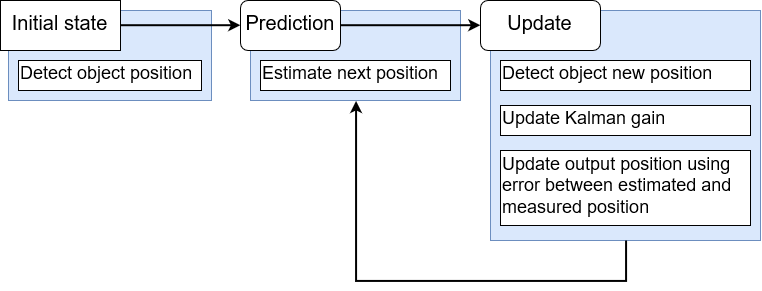
\includegraphics[width=1\textwidth]{chapter2/images/kalman_workflow.png}
		\caption{ผังการทำงานของระบบติดตามการเคลื่อนไหวของวัตถุแบบ kalman filter}
    	\label{fig:kalman_concept}
\end{figure}

ซึ่งในแต่ละช่วงการทำงานนั้นจะมีรายละเอียดดังนี้
\begin{enumerate}
	\setlength\itemsep{-0.25em}
	\item Initialize ในขั้นตอนนี้จะเป็นการกำหนดค่าเริ่มต้นให้กับเมทริกซ์สถานะหรือ state (x) และเมทริกซ์ความแปรปรวนหรือ covariance matrix (P) โดยที่เมทริกซ์สถานะจะใช้ในการเก็บข้อมูลที่ต้องการติดตามการเคลื่อนไหว 
	และเมทริกซ์ความแปรปรวนเป็นเมทริกซ์ที่ใช้บอกความแม่นยำของการทำนาย หากสามารถกำหนดค่าในเมทริกซ์ได้อย่างเหมาะสมจะทำให้การปรับปรุงประสิทธิภาพของ kalman filter ในช่วง update เสถียรเร็วขึ้น
	หลังจากได้ตำแหน่งจุดกึ่งกลางของวัตถุในเฟรมแรกแล้วจะสามารถเขียนเมทริกซ์สถานะ และเมทริกซ์ความแปรปรวนได้ดังนี้
	\begin{equation*}
		x_0 = [c_x\ c_y\ v_x\ v_y]^T
	\end{equation*}
	\begin{equation*}
		P_0 = \begin{bmatrix}
			1& 0& 0& 0\\
			0& 1& 0& 0\\
			0& 0& 1& 0\\
			0& 0& 0& 1
			\end{bmatrix}
	\end{equation*}
	\clearpage
	โดยที่ 
	\begin{conditions}
		x_0		&	เมทริกซ์สถานะ ณ เฟรมแรก\\
		c		&	จุดกึ่งกลางของวัตถุในภาพ\\
		v		&	ความเร็วในแกนที่กำหนด\\
		P_0		&	เมทริกซ์ความแปรปรวน ณ เฟรมแรก
	\end{conditions}
	จากตัวอย่างด้านบนจะเห็นว่าสิ่งที่สนใจนั้นเป็นตัวแหน่งของวัตถุ $(c_x, c_y)$ แต่ลำพังเพียงแค่ตำแหน่งไม่สามารถใช้ในการบอกตำแหน่งถัดไปได้จึงต้องใช้ความเร็วในแต่ละแกน $(v_x, v_y)$ 
	ในการหาตำแหน่งถัดไปของวัตถุ และได้กำหนดเมทริกซ์ความแปรปรวนให้เป็นเมทริกซ์เอกลักษณ์ (identity matrix)
	\item Prediction ในขั้นตอนนี้จะเป็นการทำนายตำแหน่งหรือเมทริกซ์สถานะ $(x)$ และปรับเมทริกซ์ความแปรปรวน $(P)$ โดยใช้ข้อมูลจากเฟรมก่อนหน้าเป็นพื้นฐานในการคำนวณ 
	ซึ่งมีสมการดังนี้ 
	\begin{equation}
		x' = Fx + u
		\label{equa:estimate_state}
	\end{equation}
	\begin{equation}
		P' = FPF^T + Q
	\end{equation}
	โดยที่
	\begin{conditions}
		x'		&	เมทริกซ์สถานะในเวลาถัดไปที่ได้จากการทำนาย\\
		F		&	เมทริกซ์ปรับสถานะ (state transition matrix)\\
		u		&	แรงกระทำจากภายนอกที่มีผลต่อการเคลื่อนที่ของวัตถุ (แรงเสียดทานหรือแรงลม)\\
		Q		&	เมทริกซ์ความแปรปรวนที่สอดคล้องกับข้อมูลรบกวนของสถานะ
	\end{conditions}
	จากสมการที่ \ref{equa:estimate_state} แรงกระทำจากภายนอกที่มีผลต่อการเคลื่อนที่ของวัตถุ ($u$) นั้นไม่สามารถหาได้จากภาพทำให้ต้องตัดออกไป จะทำให้สมการเหลือเพียง $x' = Fx$ 
	ซึ่งเมทริกซ์ปรับสถานะ ($F$) สามารถกำหนดให้สอดคล้องกับเมทริกซ์สถานะที่กำหนดไว้ สามารถเขียนตัวอย่างของเมทริกซ์ปรับสถานะได้ดังนี้
	\begin{equation*}
		F = \begin{bmatrix}
			1& 0& dt& 0\\
			0& 1& 0& dt\\
			0& 0& 1& 0\\
			0& 0& 0& 1
		\end{bmatrix}
	\end{equation*}
	โดย $dt$ หมายถึงความต่างของเวลาจากเฟรมก่อนหน้าถึงเฟรมปัจจุบัน จากตัวอย่างเมทริกซ์ปรับสถานะด้านบนสามารถกล่าวได้ว่าความเร็วในการเคลื่อนไหวของวัตถุนั้นคงที่ 
	เนื่องจากการกำหนดเมทริกซ์ปรับสถานะให้เป็น 1 เมื่อนำเมทริกซ์ปรับสถานะไปคูณกับเมทริกซ์สถานะจะทำให้ได้เมทริกซ์สถานะที่ได้จากการทำนาย ($x'$) ดังตัวอย่างด้านล่าง
	\begin{equation*}
		x' = \begin{bmatrix}
			1& 0& dt& 0\\
			0& 1& 0& dt\\
			0& 0& 1& 0\\
			0& 0& 0& 1
		\end{bmatrix} \begin{bmatrix}
			c_x\\ c_y\\ v_x\\ v_y
		\end{bmatrix} = \begin{bmatrix}
			c_x + v_xdt\\ c_y + v_ydt\\ v_x\\ v_y
		\end{bmatrix}
	\end{equation*}
	จากนั้นจะทำการคำนวณหาเมทริกซ์ความแปรปรวนในเวลาถัดไป ($P'$) โดยใช้เมทริกซ์ความแปรปรวนที่สอดคล้องกับข้อมูลรบกวนของสถานะ ($Q$) ในการปรับประสิทธิภาพของการทำนายสถานะถัดไปของวัตถุ 
	ซึ่งมักจะถูกกำหนดให้เป็นเมทริกซ์เอกลักษณ์ (identity matrix) ที่มีขนาดเท่ากันกับเมทริกซ์ $P$ ทั้งนี้ก็ขึ้นอยู่กับระบบของผู้ใช้
	\item Update ในขั้นตอนนี้จะเกิดขึ้นหลังจากมีการวัดค่า (measurement) ครั้งใหม่เข้ามาเพื่อนำข้อมูลที่ได้จากการวัดค่ามาเทียบกับข้อมูลที่ได้จากขั้นตอน prediction เพื่อคำนวณหาความคลาดเคลื่อน 
	และปรับตัวแปรต่างๆให้มีความเสถียรมากขึ้น โดยมีจะมีการคำนวณหาเมทริกซ์สถานะและเมทริกซ์ความแปรปรวนที่ผ่านการปรับแล้วด้วยสมการดังนี้
	\begin{equation}
		x = x' + Ky
		\label{equa:new_state}
	\end{equation}
	\begin{equation}
		P = (I-KH)P'
		\label{equa:new_covariance}
	\end{equation}
	โดยที่
	\begin{conditions}
		K		&	Kalman gain\\
		y		&	ค่าความคลาดเคลื่อนระหว่างสถานะที่ได้จากการวัดค่ากับสถานะที่ได้จากการทำนาย\\
		H		&	เมทริกซ์สำหรับปรับขนาด\\
		I		&	เมทริกซ์เอกลักษณ์
	\end{conditions}
	จากสมการที่ \ref{equa:new_state} คือการนำสถานะที่ได้จากการทำนาย และค่าความคลาดเคลื่อนระหว่างสถานะที่ได้จากการวัดค่ากับสถานะที่ได้จากการทำนายที่ผ่านการคูณด้วย Kalman gain ($K$) 
	เพื่อปรับเมทริกซ์สถานะของเวลาถัดไปให้ใกล้เคียงกับค่าที่วัดได้ให้มากขึ้น ซึ่งค่าความคลาดเคลื่อนสามารถหาได้จากสมการที่ \ref{equa:error} โดยที่ $H$ คือเมทริกซ์สำหรับปรับขนาดเพื่อทำให้เมทริกซ์สถานะที่ได้จากการทำนาย
	สามารถบวกกับเมทริกซ์สถานะที่ได้จากการวัดค่าได้ เนื่องจากเมทริกซ์สถานะที่ได้จากการวัดค่านั้นมักจะมีขนาดไม่เท่ากันกับเมทริกซ์สถานะที่ได้จากการทำนาย และ Kalman gain สามารถหาได้จากสมการที่ \ref{equa:kalmangain}

	\begin{equation}
		y = z - Hx'
		\label{equa:error}
	\end{equation}
	\begin{equation}
		K = P'H^TS^{-1}
		\label{equa:kalmangain}
	\end{equation}
	โดยที่เมทริกซ์ $S$ หาได้จากการนำเมทริกซ์ความแปรปรวนในเวลาถัดไปมารวมกับเมทริกซ์ของข้อมูลรบกวน (noise) โดยเมทริกซ์ของข้อมูลรบกวนนั้นผู้ใช้ต้องกำหนดขึ้นมาให้สอดคล้องกับระบบ 
	หากยกตัวอย่างในการตรวจจับการเคลื่อนไหวของวัตถุในสิดีโอ ข้อมูลรบกวนจะเป็นตำแหน่งแกน $x$ และแกน $y$ ของวัตถุเป็นต้น โดยสมการสำหรับหาค่าของเมทริกซ์ $S$ จะเป็นดังสมการที่ \ref{equa:Smatrix}
	\begin{equation}
		S = HP'H^T + R
		\label{equa:Smatrix}
	\end{equation}
	หลังจากปรับเมทริกซ์สถานะแล้วต่อไปคือการปรับเมทริกซ์ความแปรปรวนโดยใช้เมทริกซ์ความแปรปรวนในเวลาถัดไป และ Kalman gain ในการปรับให้เหมาะสมกับข้อมูลที่ได้จากการวัดค่ามา 
	เพื่อเพิ่มประสิทธิภาพในการติดตามตำแหน่งของวัตถุให้ใกล้เคียงกับความเป็นจริงให้มากขึ้น โดยสมการจะเป็นดังในสมการที่ \ref{equa:new_covariance}
\end{enumerate}
\begin{figure}[!ht]
	\centering
	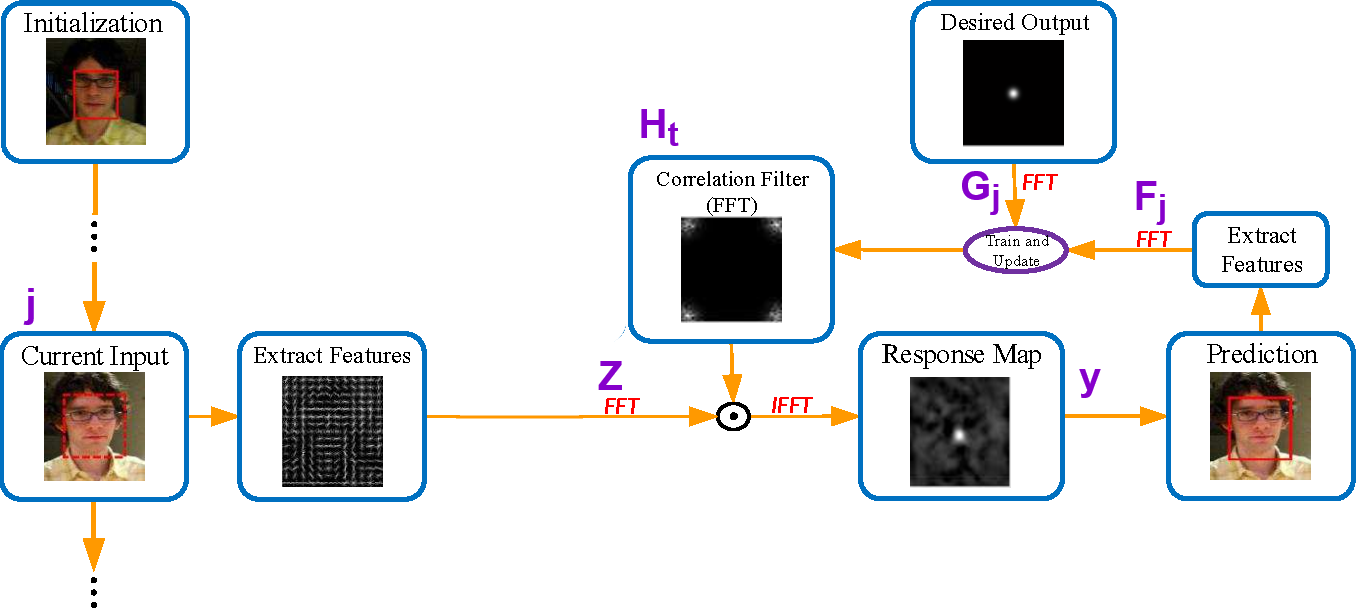
\includegraphics[width=1\textwidth]{chapter2/images/correlation_marked.png}
		\caption[ผังการทำงานของระบบติดตามการเคลื่อนไหวของวัตถุแบบ correlation filter]{ผังการทำงานของระบบติดตามการเคลื่อนไหวของวัตถุแบบ correlation filter\textsuperscript{\cite{chen2015experimental}}}
    	\label{fig:correlation_concept}
\end{figure}

จากรูปที่ \ref{fig:correlation_concept} เป็นขั้นตอนการทำงานของระบบติดตามการเคลื่อนไหวของวัตถุแบบ correlation filter ซึ่งการทำงานจะมีสามขั้นตอนหลักๆเหมือนกันกับ Kalman filter คือ
initialize, prediction และ update โดยในแต่ละขั้นตอนจะมีรายละเอียดดังนี้
\begin{enumerate}
	\item Initialize ในขั้นตอนนี้จะทำการใช้โมเดลปัญญาประดิษฐ์ในการตรวจจับวัตถุที่สนใจภายในเฟรมแรกของวิดีโอเพื่อหาตำแหน่งและกรอบสี่เหลี่ยมของวัตถุนั้น 
	จากนั้นนำภาพที่อยู่ในกรอบสี่เหลี่ยมไปผ่านกระบวนการแปลงฟูรีเยร์ (fourier transform) เพื่อใช้เป็นผลลัพธ์ที่ต้องการ (desired output) ($G_j$) สำหรับใช้ในการสร้าง correlation filter ในเฟรมถัดไป ($H_t$)
	\item Prediction หลังจากได้รับภาพใหม่ ($j$) เข้ามาจะทำการสกัดผังคุณลักษณะ ซึ่งทั้งนี้ก็แล้วแต่ว่าผู้พัฒนาต้องการใช้อะไรในการสกัดผังคุณลักษณะของภาพออกมา 
	หลังจากได้ผังคุณลักษณะของภาพที่เข้ามาใหม่แล้วก็นำไปผ่านกระบวนการแปลงฟูรีเยร์ ($Z$) ก่อนจะไล่ทำกระบวนการ element-wise ด้วย correlation filter แล้วทำการแปลงฟูรีเยร์ผกผัน (inverse fourier transform)
	จนครบทั้งภาพเพื่อหาผังการตอบสนองของเฟรมปัจจุบัน (response map) ($y$) ที่มีค่ามากที่สุดออกมา โดยผังการตอบสนองที่มีค่ามากที่สุดจะเป็นตำแหน่งถัดไปของวัตถุที่สนใจ ซึ่งสามารถเขียนเป็นสมการได้ดังนี้
	\begin{equation}
		y = \mathbb{F}^{-1}\{\bar{H_t}\star Z\}
	\end{equation}
	โดยที่
	\begin{conditions}
		y				&	ผังการตอบสนอง\\
		\mathbb{F}^{-1}	&	การแปลงฟูรีเยร์ผกผัน\\
		\bar{H_t}		&	correlation filter ที่ผ่านการทำ complex conjugation มาแล้ว\\
		\star			&	element-wise operator\\
		Z				&	ผังคุณลักษณะที่ผ่านกระบวนการแปลงฟูรีเยร์มาแล้ว
	\end{conditions}
	\clearpage
	\item Update หลังจากทำนายตำแหน่งของวัตถุในภาพใหม่ได้แล้วจะทำการตัดภาพในกรอบสี่เหลี่ยมใหม่มาสกัดคุณลักษณะแล้วทำกระบวนการแปลงฟูรีเยร์ ($F_j$) และผลลัพธ์ที่ต้องการจากเฟรมก่อนหน้า ($G_j$) 
	ไปผ่านกระบวนการตามสมการที่ \ref{equa:correlation} เพื่อปรับ correlation filter ให้เปลี่ยนไปตามเหตุการณ์ที่เกิดขึ้นในเฟรมวิดีโอ 
	แล้วทำการแทนที่ผลลัพธ์ที่ต้องการจากเฟรมก่อนหน้าด้วยผังการตอบสนองของเฟรมปัจจุบัน จะทำให้การทำนายตำแหน่งในเฟรมต่อๆไปมีประสิทธิภาพมากขึ้นเนื่องจากมีการปรับปรุงตัวกรองให้เป็นปัจจุบันตลอดเวลา
	\begin{equation}
		H_t = \frac{\bar{G_j}F_j}{\bar{F_j}F_j}
		\label{equa:correlation}
	\end{equation}
\end{enumerate}